\documentclass[12pt, a4paper]{article}
\usepackage{lmodern}
%\usepackage[margin=1cm]{geometry}
\usepackage{pdflscape}
\usepackage{color}
\usepackage{footnote}
\usepackage{graphicx}
%\pagestyle{empty}
\newcommand{\cell}[2][c]{%
  \begin{tabular}[#1]{@{}c@{}}#2\end{tabular}}
\newcommand{\rowhead}[2]{\cell{\color{red}#1\\ \color{green}#2}}
\newcommand{\cont}[5]{\cell{\color{red}#1\\ \color{blue}#2\\ #3\\ #4\\ \color{green}#5}}
\newcommand{\deprecont}[5]{\cell{\color{red}#1\\ \color{blue}#2\\ #3\\ #4\\ \color{green}#5\\ \color{red}Deprecated warning}}
\newcommand{\noacc}{No accumulation}
\newcommand{\acc}{Accumulation}
\newcommand{\noconv}{No conversion}
\newcommand{\sca}{Scaling possible}
\newcommand{\nosca}{Scaling not possible}
\newcommand{\conv}{Conversion}
\newcommand{\serfal}{Service=false}
\newcommand{\sertru}{Service=true}
\newcommand{\err}{\color{red}Error}
\newcommand{\depre}{\color{red}Deprecated}
\newcommand{\follsup}{Following supports $S_{R+1}\dots S_i\dots S_N$}
\newcommand{\allsup}{All supports $S_1\dots S_i\dots S_N$}
\newcommand{\modlen}{moduleLength}
\newcommand{\modsur}{moduleSurface}
\newcommand{\nummod}{numModules}
\newcommand{\suplen}{supportLength}
\newcommand{\supsur}{supportSurface}
\newcommand{\tkl}{tkLayout}


\begin{document}
\section{Introduction to material model}
The material inside \tkl is present inside the modules (i.e. silicon
and cooling blocks),
and outside the modules (i.e. cables or cooling pipes). Is possible to
specify, in the configuration files, the material inside:
\begin{itemize}
\item modules;
\item rods (the ladders);
\item barrel's layers;
\item endcap's disks;
\item custom cylinders and disks (i.e. for the supports).
\end{itemize}
Is also possible to set material from every element:
\begin{itemize}
\item locally,
\item exiting.
\end{itemize}

\begin{figure}[h]
  \centering
  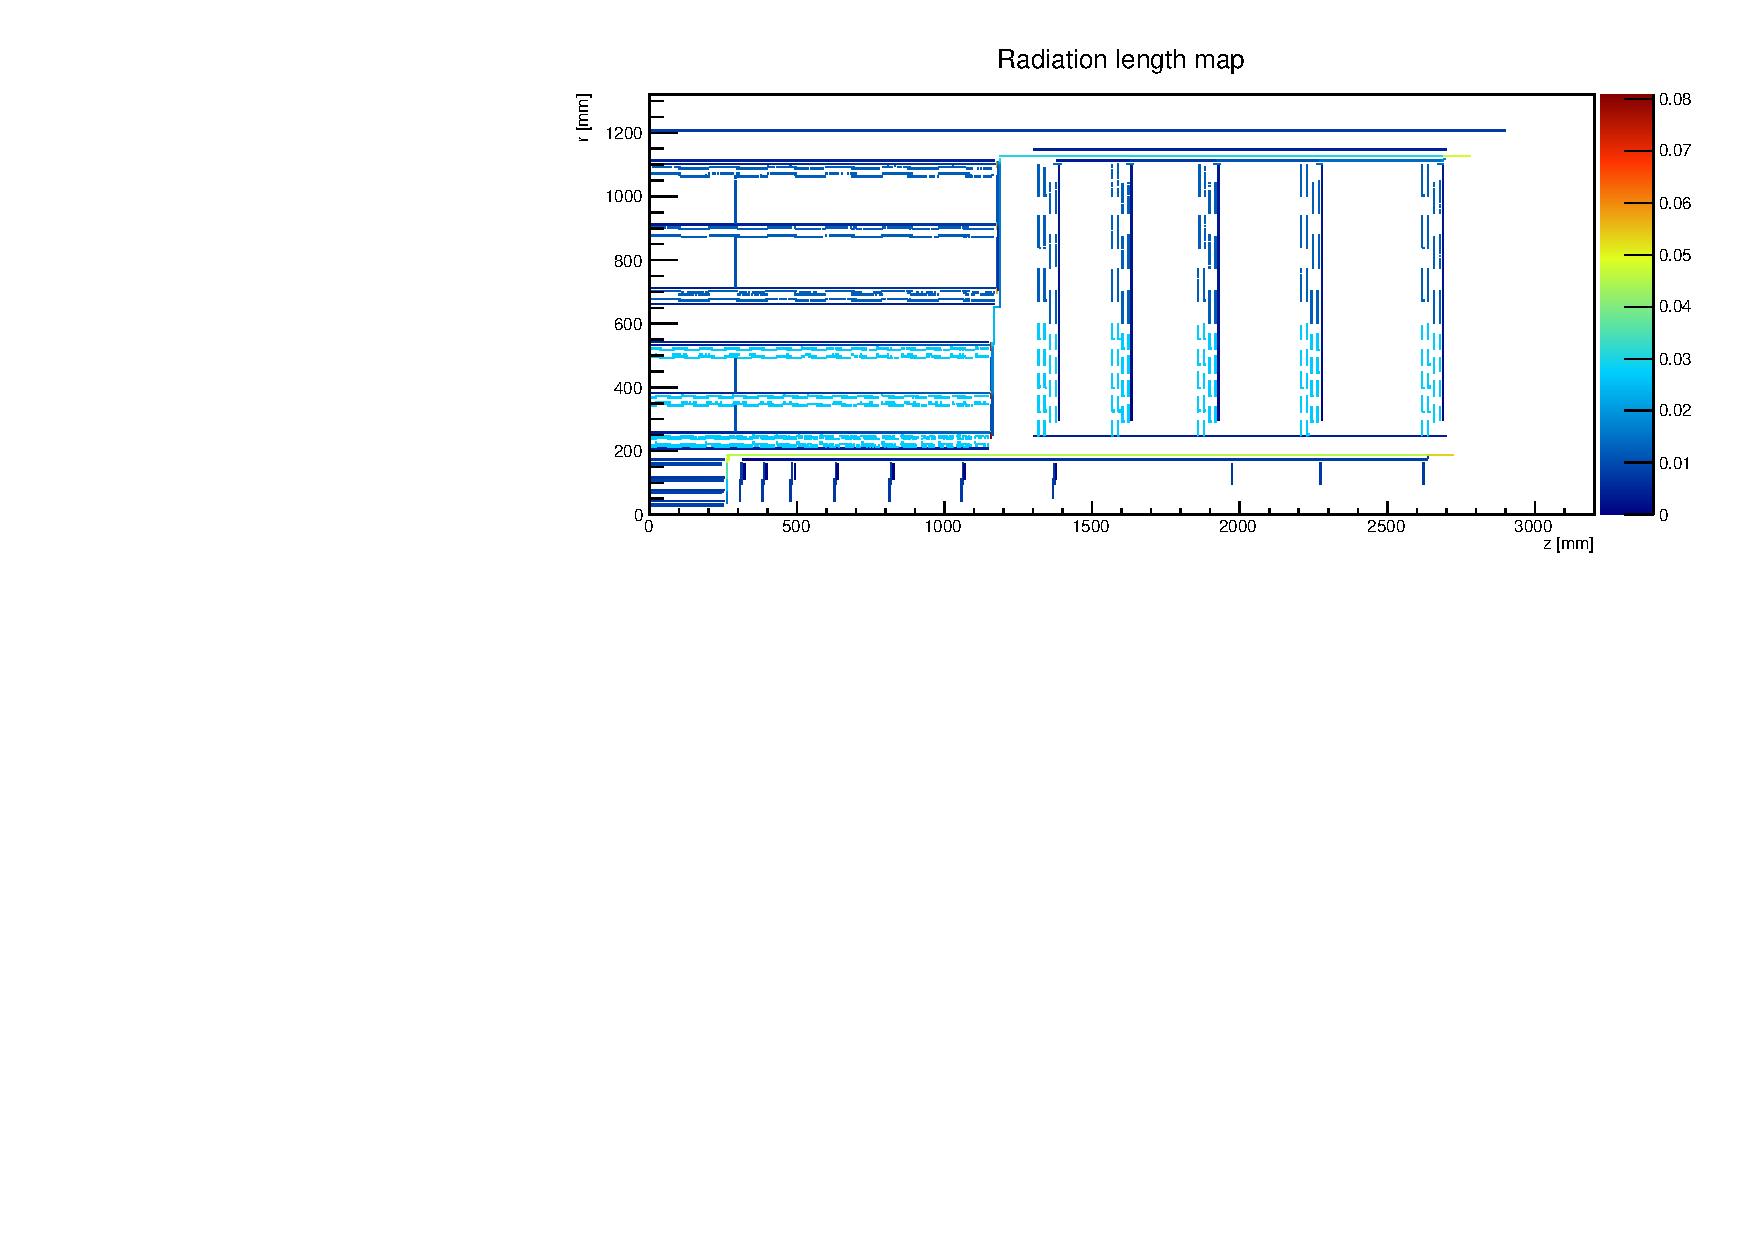
\includegraphics[width=\textwidth]{img/materialMap.pdf}  
  \caption{Material routing}
  \label{fig:materialMap}
\end{figure}

Apart from the material is possible also to define \emph{conversions}
in special points: at the end of the layers, at the end of the disks,
and in custom positon along the way.

In figure~\ref{fig:materialMap}
is visible the material for the modules and the \emph{sections} for
the routing of the material, section~\ref{sec:userManual} deal with
the description in detail of how to build the configuration files and
how the material is distributed, from an user point of view.

The material \emph{routing algorithm} builds automatically all the necessary structures for
keeping all the materials that not belongs to the modules. It builds
\emph{sections} on top of the layers, and on the right of the disks,
then connect those sections for each barrel and endcap, then connect
barrels and endcaps with the cable exit point (upper right point of
tracker). Section~\ref{sec:developerManual} deal with the description
in detail of the routing algorithm from a developer point of view.




\section{User manual}\label{sec:userManual}
\subsection{Material routing effects}
The first column is where the material is defined and if is defined
with \emph{service} true or false. The other columns are the different
effect regarding the unit of measure of the material, for each cell:
the first field is the destination volume; the second is the amount of
material in grams; the third specify if the material is accumulating
along the layer/disk; the fourth specify if the material is converted
after the layer/disk or only stay in the layer/disk; the fifth if is
possible or not to set the scaling on channels.
\begin{landscape}
  \begin{savenotes}
    \begin{center}
      \fontsize{7pt}{8.3}\selectfont
      \begin{tabular}{|c||c|c|c|}
        \hline
        & \color{green}Unit=$g/m$ & \color{green}Unit=$mm$ & \color{green}Unit=$g$\\
        \hline\hline
        \rowhead{Module}{\serfal} & \cont{Module}{$\times \modlen$}{\noacc}{\noconv}{\sca}& \cont{Module}{$\times \modsur\times \rho$ (sensor surface)}{\noacc}{\noconv}{\sca}& \cont{Module}{$\times 1$}{\noacc}{\noconv}{\sca}\\
        \hline
        \rowhead{Module in ring $R$\footnote{of $N$ rings}}{\sertru\footnote{\label{sertrunote}may be converted by station}} & \cont{\follsup}{$\times \nummod_R \times \suplen_i$}{\acc}{\conv (1:1 by default, with warning)}{\sca} & \deprecont{\follsup}{$\times \nummod_R \times \supsur_i \times \rho$}{\acc}{\conv  (1:1 by default, with warning)}{\sca} & \err \\
        \hline
        \rowhead{Rod (barrel\footnote{line of one module per ring with same $\phi$})}{\serfal} & \cont{\allsup}{$\times \nummod_1 \times \suplen_i$}{\noacc}{\noconv}{\nosca} & \cont{\allsup}{$\times \supsur_i \times \rho$}{\noacc}{\noconv}{\nosca} & \cont{\allsup}{$\times \nummod_1 \times \frac{\suplen_i}{\sum_{j=1}^N\suplen_j}$}{\noacc}{\noconv}{\nosca} \\
        \hline
        \rowhead{Rod (barrel)}{\sertru\textsuperscript{\ref{sertrunote}}} & \cont{\allsup}{$\times \nummod_1 \times \suplen_i$}{\noacc}{\conv}{\nosca} & \deprecont{\allsup}{$\times \supsur_i \times \rho$}{\noacc}{\conv}{\nosca} & \err \\
        \hline
        \rowhead{Layer/Disk}{\serfal} & \cont{\allsup}{$\times \suplen_i$}{\noacc}{\noconv}{\nosca} & \cont{\allsup}{$\times \supsur_i \times \rho$}{\noacc}{\noconv}{\nosca} & \cont{\allsup}{$\times \frac{\suplen_i}{\sum_{j=1}^N\suplen_j}$}{\noacc}{\noconv}{\nosca} \\
        \hline
        \rowhead{Layer/Disk}{\sertru\textsuperscript{\ref{sertrunote}}} & \cont{\allsup}{$\times \suplen_i$}{\noacc}{\conv}{\nosca} & \deprecont{\allsup}{$\times \supsur_i \times \rho$}{\noacc}{\conv}{\nosca} & \err \\
        \hline
      \end{tabular}
    \end{center}
    \begin{center}
      \tiny
      \begin{tabular}{|c|c|c|c|}
        \hline
        & Modules & Cylind. service sections & disk service section \\
        \hline
        Length & Local $y$ & $\Delta z$ & $\Delta r$ \\
        \hline
        Surface & Sensor surface & $2\pi r \Delta z$ & $\pi({r_2}^2 - {r_1}^2)$ \\
        \hline
      \end{tabular}
    \end{center}
  \end{savenotes}
\end{landscape}



\section{Developer manual}\label{sec:developerManual}

\subsection{General algorithm description}






\subsection{Classes description}

\subsubsection{namespace insur}

\begin{itemize}

\item MaterialBudget
\item MaterialProperties
\item MaterialTable
\item BaseMaterial
\item MaterialTable2
\item ElementaryMaterial : public BaseMaterial
\item CompositeMaterial : public BaseMaterial
\item InactiveElement : public MaterialProperties
\item InactiveRing : public InactiveElement
\item InactiveSurfaces
\item InactiveTube : public InactiveElement
\item MatCalc

\end{itemize}



\subsubsection{namespace material}

\begin{itemize}

\item MaterialObject : public PropertyObject
\item MaterialObject::ReferenceSensor : public PropertyObject
\item MaterialObject::MaterialObjectKey
\item MaterialObject::Element : public PropertyObject
\item MaterialObject::Component : public PropertyObject
\item MaterialObject::Materials : public PropertyObject
\item MaterialSection : public MaterialObject
\item MaterialStation : public MaterialSection
\item MaterialTab : public MaterialTabType
\item Materialway
\item Materialway::RodSectionsStation
\item Materialway::Section
\item Materialway::Station : public Materialway::Section
\item Materialway::Boundary
\item Materialway::OuterUsher
\item Materialway::InnerUsher
\item Materialway::ModuleUsher
\item ConversionStation : public MaterialObject
\item ConversionStation::Inoutput : public PropertyObject
\item ConversionStation::Conversion : public PropertyObject
\item WeightDistributionGrid : public WeightDistributionGridMapType

\end{itemize}



\end{document}


